\documentclass{article}
\usepackage{fleqn}
\usepackage{epsf}
\usepackage{aima2e-slides}
\usepackage{graphicx}

\usepackage[landscape]{geometry}

%\usepackage{amsmath}
\usepackage{amssymb}

\newcommand{\mm}{\!\!-\!\!}
\newcommand{\prompt}{$> \ $}
\newcommand{\rep}[1]{\ulcorner #1 \urcorner}

\begin{document}

\begin{huge}
\titleslide{Chapter 3. Expressions \\ (Essentials of Programming Languages)}{Kwanghoon Choi \\ \ \\ Software Languages and Systems Laboratory\\ Chonnam National University}

\sf

%%%%%%%%%%%% Slide %%%%%%%%%%%%%%%%%%%%%%%%%%%%%%%%%%%%%%%%%%%%%%%%%%%
\heading{Outline}


To study the binding and scoping of variables, we introduce a series of small languages to illustrate the concepts, \al
- writing specifications for the languages, and \al
- implemeting them using interpreters

\blob Specification and Implementation Strategy

\blob LET: A Simple Language

\blob PROC: A Language with Procedures

\blob LETREC: A Language with Recursive Procedures

\blob Scoping and Binding of Variables

\blob Eliminating Variable names \& Implementing Lexical Addressing

%%%%%%%%%%%% Slide %%%%%%%%%%%%%%%%%%%%%%%%%%%%%%%%%%%%%%%%%%%%%%%%%%%
\heading{3.1 Specification and Implementation Strategy}

Our specification will consist of assertions of the form \al
- (value-of $exp$ $\rho$) = $val$ \al
meaning the value of expression $exp$ in environment $\rho$ is $val$.

The overall picture of our implementation \al
- A figure in the next slide \al
- Front-end: scanning (lexical analylsis), parsing (syntax analysis) \al
- Parser generator \al
  : (Input) a lexical specification and a grammar \al
  : (Output) a scanner and a parser

%%%%%%%%%%%% Slide %%%%%%%%%%%%%%%%%%%%%%%%%%%%%%%%%%%%%%%%%%%%%%%%%%%
\heading{3.1 Spec. and Impl. Strategy(cont.)}

The overall picture of our implementation

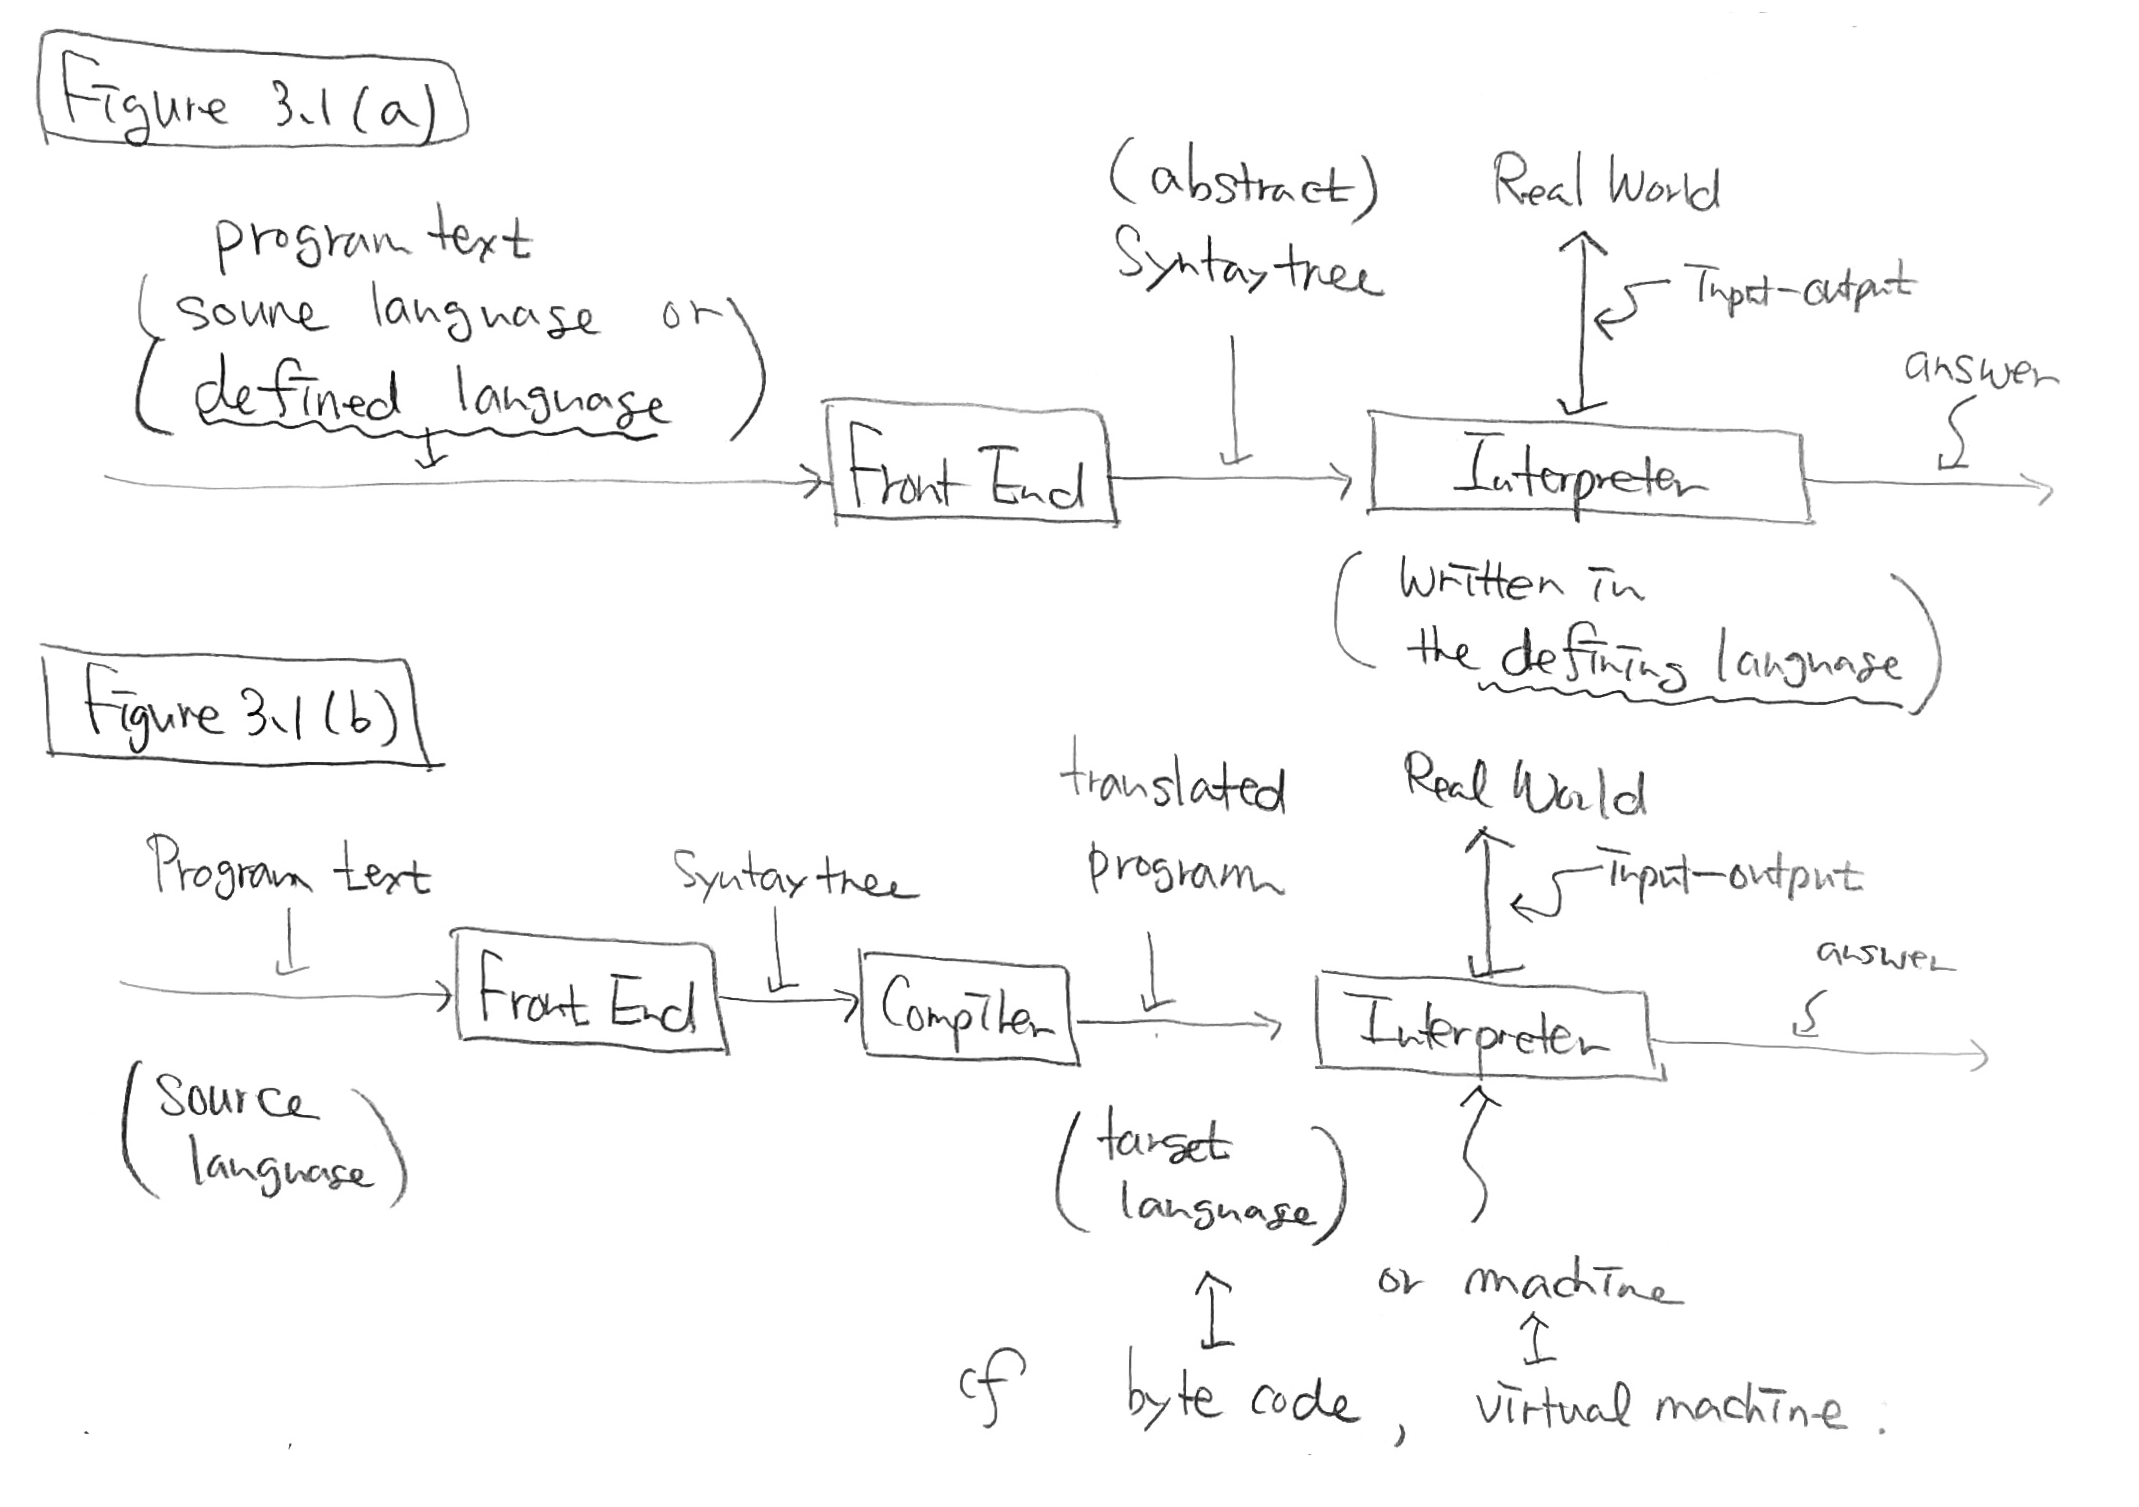
\includegraphics[width=0.85\linewidth]{fig_3_1_lang_proc_system}

%%%%%%%%%%%% Slide %%%%%%%%%%%%%%%%%%%%%%%%%%%%%%%%%%%%%%%%%%%%%%%%%%%
\heading{3.2 LET: A Simple Language}

Four programs (expressions) written in LET: \al
\al
- (-(x,3), -(v,i)) \al
\al
if zero? (-(x,11)) then -(y,2) else -(y,4) \al
\al
let x = 5 in -(x, 3) \al
\al
let z = 5 in let x = 3 in let y = -(x, 1) in let x = 4 in -(z, -(x,y))

%%%%%%%%%%%% Slide %%%%%%%%%%%%%%%%%%%%%%%%%%%%%%%%%%%%%%%%%%%%%%%%%%%
\heading{3.2.1 Specifying the Syntax}

Syntax for the LET language \al
\al
Program ::= Expression \fbox{a-program (exp1)} \al
\al
Expression :: = Number \fbox{const-exp (num)} \al
Expression ::= -(Expression , Expression) \fbox{diff-exp (exp1 exp2)} \al
Expression ::= zero? (Expression) \fbox{zero?-exp (exp1)} \al
Expression ::= if Expression then Expression else Expression \al 
\ \ \ \ \ \ \ \ \ \fbox{if-exp (exp1 exp2 exp3)} \al
Expression ::= Identifier \fbox{var-exp (var)} \al
Expression ::= let Identifier = Expression in Expression \al
\ \ \ \ \ \ \ \ \ \fbox{let-exp (var exp1 body)}
\al
\al
cf. Concrete syntax \fbox{Abstract syntax}

%%%%%%%%%%%% Slide %%%%%%%%%%%%%%%%%%%%%%%%%%%%%%%%%%%%%%%%%%%%%%%%%%%
\heading{3.2.2 Specification of Values}

Each programming language has at least two set of values \al
- Expressed values: the possible values of expressions \al
- Denoted values: the values bound to variables

Values and interfaces in the LET language,
%\mat{
\begin{eqnarray*}
ExpVal & ::= & Int + Bool \\
DenVal & ::= & Int + Bool
\end{eqnarray*}
%} 
\al
- num-val : $Int \rightarrow ExpVal$ \al
- bool-val : $Bool \rightarrow ExpVal$ \al
- expval-\textgreater num : $ExpVal \rightarrow Int$ \al
- expval-\textgreater bool : $ExpVal \rightarrow Bool$ 

%%%%%%%%%%%% Slide %%%%%%%%%%%%%%%%%%%%%%%%%%%%%%%%%%%%%%%%%%%%%%%%%%%
\heading{3.2.3 Environments}

Environments keep track of the meaning of each variable in the expression benig evaluated.

Some abbreviations in writing environments\al
- $[x=3] \ [y=7] \ [u=5]\rho$ \al
\ \ denotes (extend-env `x 3 (extend-env `y 7 (extend-env `u 5 $\rho$))).

Formally, \al
- $\rho$ ranges over environments \al
- $[]$ denotes the empty environments \al
- $[var=val]\rho$ denotes (extend-env $var$ $val$ $\rho$) \al
- $[var_1=val_1,var_2,=val_2]\rho$ abbreviates $[var_1=val_1]([var_2=val_2]\rho)$ \al
- $[var_1=val_1,\cdots, var_n,=val_n]$ denotes the environment in which the value of $var_1$ is $val_1$, etc.

%%%%%%%%%%%% Slide %%%%%%%%%%%%%%%%%%%%%%%%%%%%%%%%%%%%%%%%%%%%%%%%%%%
\heading{3.2.4 Specifying the Behavior of Expressions}

Constructor interfaces \al
- const-exp : $Int \rightarrow Exp$ \al
- zero?-exp : $Exp \rightarrow Exp$ \al
- if-exp : $Exp \times Exp \times Exp \rightarrow Exp$ \al
- diff-exp : $Exp \times Exp \rightarrow Exp$ \al
- var-exp : $Var \rightarrow Exp$ \al
- let-exp : $Var \times Exp \times Exp \rightarrow Exp$ \al
(See Figure 3.2)

Observer interfaces \al
- value-of : $Exp \times Env \rightarrow ExpVal$ \al
(Recall : value-of $exp$ $\rho$ = $val$)

%%%%%%%%%%%% Slide %%%%%%%%%%%%%%%%%%%%%%%%%%%%%%%%%%%%%%%%%%%%%%%%%%%
\heading{3.2.4 Specifying the Behavior of Exprs (Cont.)}

Before starting on an implementation, we write down a specification
for the behaviors of the procedures in the previous slide \al
\al
(value-of (const-exp $n$) $\rho$) = (num-val $n$) \al
\al
(value-of (var-exp $var$) $\rho$) = (apply-env $\rho$ $var$) \al
\al
(value-of (diff-exp $exp_1$ $exp_2$) $\rho$) = \al
\ \ \ (num-val \al
\ \ \ \ \ \ (- \al
\ \ \ \ \ \ \ \ \ (expval-\textgreater num (value-of $exp_1$ $\rho$)) \al
\ \ \ \ \ \ \ \ \ (expval-\textgreater num (value-of $exp_2$ $\rho$))))

(See Figure 3.3 for ``an execution of'' this specification)

%%%%%%%%%%%% Slide %%%%%%%%%%%%%%%%%%%%%%%%%%%%%%%%%%%%%%%%%%%%%%%%%%%
\heading{3.2.5 Specifying the Behavior of Programs}

In the LET language, a whole program is just an expression. \al
\al
(value-of-program $exp$) = (value-of $exp$ $\rho_{initial}$)


%%%%%%%%%%%% Slide %%%%%%%%%%%%%%%%%%%%%%%%%%%%%%%%%%%%%%%%%%%%%%%%%%%
\heading{3.2.6 Specifying Conditionals}

The LET language has one constructor of boolean, zero?, and one observer
of booleans, the if expression.

\begin{tabular}{l}
(value-of $exp_1$ $\rho$) = $val_1$ \\ \hline
(value-of (zero?-exp $exp_1$ $\rho$) \\
\ \ \ 
$= \left \{
	\begin{array}{l}
	\mbox{(bool-val \#t) \ \ \ if (expval-\textgreater num $val_1$) $=$ 0} \\
	\mbox{(bool-val \#f) \ \ \ if (expval-\textgreater num $val_1$) $\not=$0}
	\end{array}
	\right .$ 
\end{tabular}


\begin{tabular}{l}
(value-of $exp_1$ $\rho$) = $val_1$ \\ \hline
(value-of (if-exp $exp_1$ $exp_2$ $exp_3$ $\rho$) \\
\ \ \ 
$= \left \{
	\begin{array}{l}
	\mbox{(value-of $exp_2$ $\rho$) \ \ \ if (expval-\textgreater num $val_1$) $=$ \#t} \\
	\mbox{(value-of $exp_3$ $\rho$) \ \ \ if (expval-\textgreater num $val_1$) $\not=$ \#f}
	\end{array}
	\right .$ 
\end{tabular}

(See Figure 3.4 for a simple calculation of a conditional expression)	

%%%%%%%%%%%% Slide %%%%%%%%%%%%%%%%%%%%%%%%%%%%%%%%%%%%%%%%%%%%%%%%%%%
\heading{3.2.7 Specifying let}

In the LET language, a let expression creates a new variable binding.

\begin{tabular}{l}
(value-of $exp_1$ $\rho$) = $val_1$ \\ \hline
(value-of (let-exp $var$ $exp_1$ $body$ $\rho$) \\
\ \ \ = (value-of $body$ $[var=val_1]\ \rho$
\end{tabular} 

%%%%%%%%%%%% Slide %%%%%%%%%%%%%%%%%%%%%%%%%%%%%%%%%%%%%%%%%%%%%%%%%%%
\heading{3.2.8 Implementing the Specification of LET}

In Scheme, a data type for abstract syntax for LET \al
(define-datatype program program? \al
\ \ \ (a-program \al
\ \ \ \ \ \ (exp1 expression?))) \al
\al
(define-datatype expression expression? \al
\ \ \ (const-exp \al
\ \ \ \ \ \ (num number?)) \al
\ \ \ (diff-exp \al
\ \ \ \ \ \ (exp1 expression?)) \al
\ \ \ \ \ \ (exp2 expression?)) \al
\ \ \ $\cdots$ \al
(See Figure 3.6)

%%%%%%%%%%%% Slide %%%%%%%%%%%%%%%%%%%%%%%%%%%%%%%%%%%%%%%%%%%%%%%%%%%
\heading{3.2.8 Implementing the Spec. of LET (Cont.)}

Our implementation uses SLLGEN as a front-end to parse,  \al
- e.g., an input text ``(- x 123)'' into  \al
\ \ (a-program (diff-exp (var-exp `x) (const-exp `123))) in Scheme

In Scheme, a data type for expressed values \al
(define-datatype expval expval? \al
\ \ \ (num-val (num number?)) \al
\ \ \ (bool-val (bool boolean?)))

(Exercise: Implement expval-\textgreater num and expval-\textgreater bool.)

We can write down the interpreter, shown in Figure 3.8 and 3.9, in Scheme \al
- run : $String \rightarrow ExpVal$ \al
- value-of-program : $Program \rightarrow Expval$ \al
- value-of : $Exp \times Env \rightarrow Expval$ 

%%%%%%%%%%%% Slide %%%%%%%%%%%%%%%%%%%%%%%%%%%%%%%%%%%%%%%%%%%%%%%%%%%
\heading{3.3 PROC: A Language with Procedures}

In PROC, one can create new procedures as: \al
\al
let f = proc (x) - (x, 11) \al
in (f (f 77)) \al
\al
(proc (f) (f (f 77))) \al
proc (x) - (x, 11) \al
\al
let x = 200 \al
in let f = proc (z) -(z, x) \al
\ \ \ in let x = 100 \al
\ \ \ \ \ \ in let g = proc (z) - (z, x) \al
\ \ \ \ \ \ \ \ \ in -((f 1), (g 1)) \al
(Note that the two identical procedures behave differently.)

%%%%%%%%%%%% Slide %%%%%%%%%%%%%%%%%%%%%%%%%%%%%%%%%%%%%%%%%%%%%%%%%%%
\heading{3.3 PROC: A Language with Procedures (Cont.)}

Procedures are new expressed values
%\mat{
\begin{eqnarray*}
ExpVal & ::= & Int + Bool + Proc \\
DenVal & ::= & Int + Bool + Proc 
\end{eqnarray*}
%}

$Proc$ is a set of values representing procedures with a constructor and an observer \al
- procedure : $Var \times Exp \times Env \rightarrow Proc$  \al
- apply-procedure : $Proc \times ExpVal \rightarrow ExpVal$ 


%%%%%%%%%%%% Slide %%%%%%%%%%%%%%%%%%%%%%%%%%%%%%%%%%%%%%%%%%%%%%%%%%%
\heading{3.3 PROC: A Language with Procedures (Cont.)}

Syntax for procedure creation and calling \al
\al
Expression :: = proc (Identifier) Expression \fbox{proc-exp (var body)} \al
Expression :: = (Expression Expression) \fbox{call-exp (rator rand)} \al
\al
\ \ \ var: bound variable or formal parameter \al
\ \ \ rator: operator \al
\ \ \ rand: operand or actual parameter \al
\ \ \ \ \ \ (argument: the value of an actual parameter)

%%%%%%%%%%%% Slide %%%%%%%%%%%%%%%%%%%%%%%%%%%%%%%%%%%%%%%%%%%%%%%%%%%
\heading{3.3 PROC: A Language with Procedures (Cont.)}

(value-of (proc-exp $var$ $body$) $\rho$) \al
\ \ \ = (proc-val (procedure $var$ $body$ $\rho$))

[Exercise] Explain what proc-val is. 

(value-of (call-exp $rator$ $rand$) $\rho$) \al
\ \ \ = (let ((proc (expval-\textgreater proc (value-of $rator$ $\rho$))) \al
\ \ \ \ \ \ \ \ \ \ \ \ \ (arg (value-of $rand$ $\rho$))) \al
\ \ \ \ \ \ \ \ \ (apply-procedure proc arg))

(apply-procedure (procedure $var$ $body$ $\rho$) $val$) \al
\ \ \ = (value-of $body$ $[var=val]\rho$)

%%%%%%%%%%%% Slide %%%%%%%%%%%%%%%%%%%%%%%%%%%%%%%%%%%%%%%%%%%%%%%%%%%
\heading{3.3.1 An Example}

[Exercise] Execute the specification defined in the previous slide 
with procedural examples.

%%%%%%%%%%%% Slide %%%%%%%%%%%%%%%%%%%%%%%%%%%%%%%%%%%%%%%%%%%%%%%%%%%
\heading{3.3.2 Representing Procedures}

In Scheme, a new data type for expressed values including proc-val \al
(define-datatype expval expval? \al
\ \ \ (num-val (num number?)) \al
\ \ \ (bool-val (bool boolean?)) \al
\ \ \ (proc-val (proc proc?)))

Two alternative implementations of proc are in the textbook. \al
- A data structure representation is explained in the next slide. \al
\ \ \ (See Section 3.3.2 for a procedural representation)

%%%%%%%%%%%% Slide %%%%%%%%%%%%%%%%%%%%%%%%%%%%%%%%%%%%%%%%%%%%%%%%%%%
\heading{3.3.2 Representing Procedures}

We define procedure as a data structure representation

(define-datatype proc proc? \al
\ \ \ (procedure \al
\ \ \ \ \ \ (var identifier?) \al
\ \ \ \ \ \ (body expression?) \al
\ \ \ \ \ \ (saved-env environment?)))

(define apply-procedure \al
\ \ \ (lambda (proc1 val) \al
\ \ \ \ \ \ (cases proc proc1 \al
\ \ \ \ \ \ \ \ \ (procedure (var body saved-env) \al
\ \ \ \ \ \ \ \ \ \ \ \ (value-of body (extend-env var val saved-env))))))

Procedures in the data structure  representation are called {\it closures}. \al
- a closed procedure + (its creation) environment

%%%%%%%%%%%% Slide %%%%%%%%%%%%%%%%%%%%%%%%%%%%%%%%%%%%%%%%%%%%%%%%%%%
\heading{3.3.2 Representing Procedures (Cont.)}

An implementation of the interpreter \al
- should extend one in Figure 3.8 and 3.9 \al
- by adding value-of two new clauses as : \al
\al
\ \ \ \ \ \ (proc-exp (var body)  \al
\ \ \ \ \ \ \ \ \ (proc-val (procedure var body env))) \al
\al
\ \ \ \ \ \ (call-exp (rator rand) \al
\ \ \ \ \ \ \ \ \ (let ((proc (expval-\textgreater proc (value-of rator env))) \al
\ \ \ \ \ \ \ \ \ \ \ \ \ \ (arg (value-of rand env))) \al
\ \ \ \ \ \ \ \ \ \ \ \ (apply-procedure proc arg)))

%%%%%%%%%%%% Slide %%%%%%%%%%%%%%%%%%%%%%%%%%%%%%%%%%%%%%%%%%%%%%%%%%%
\heading{3.4 LETREC: A Lang. with Recursive Procs.}

In LETREC, one can create a recursive procedure as: \al
\al
letrec double (x) \al
\ \ \ \ \ \ \ \ \ = if zero? (x) then 0 else - ((double -(x, 1)), -2) \al
in (double 6)

Issue: When a closure for the recursive procedure double is created,
the creation environment must contain a binding for double, 
which is the closure itself!

\begin{center}
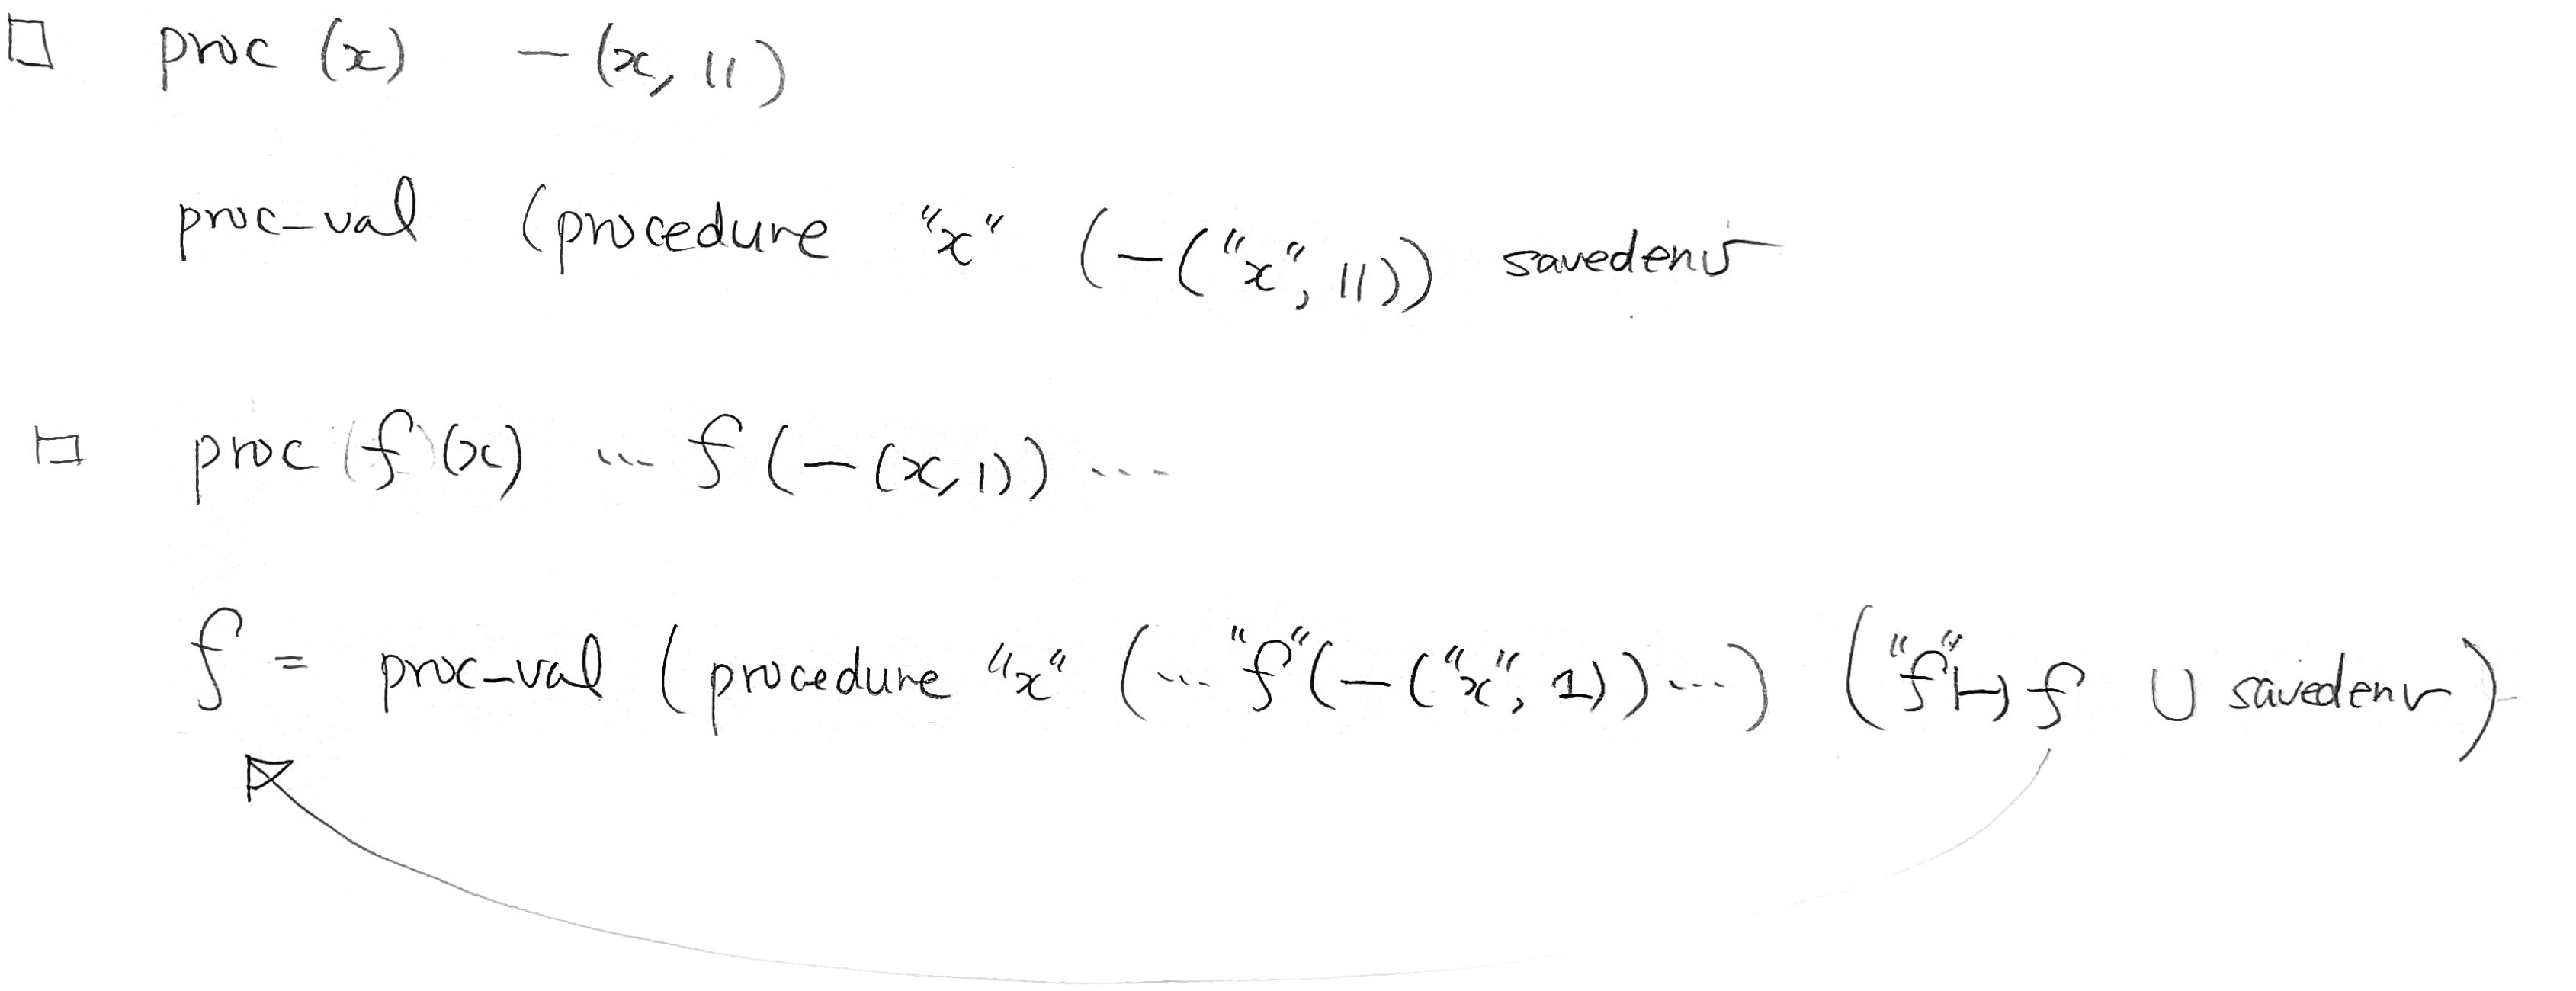
\includegraphics[width=0.7\linewidth]{rec_proc_val.jpg}
\end{center}

%%%%%%%%%%%% Slide %%%%%%%%%%%%%%%%%%%%%%%%%%%%%%%%%%%%%%%%%%%%%%%%%%%
\heading{3.4 LETREC: A Lang. with Rec. Procs. (Cont.)}

Syntax for letrec \al
\al
Expression :: =  \al
\ \ \ letrec Identifier (Identifier) = Expression in Expression \al
\ \ \  
\fbox{letrec-exp (p-name b-var p-body letrec-body)}

Specification \al
\al
(value-of \al
\ \ (letrec-exp $proc\mm name$ $bound\mm var$ $proc\mm body$ $letrec\mm body$) $\rho$) \al
\ \ \ = (value-of $lectrec\mm body$ \al
\ \ \ \ \ \ \ \ \ (extend-env-rec $proc\mm name$ $bound\mm var$ $proc\mm body$ $\rho$))

What is the specification for extend-env-rec then?

%%%%%%%%%%%% Slide %%%%%%%%%%%%%%%%%%%%%%%%%%%%%%%%%%%%%%%%%%%%%%%%%%%
\heading{3.4 LETREC: A Lang. with Rec. Procs. (Cont.)}

Assume $\rho_1$ is (extend-env-rec $proc\mm name$ $bound\mm var$ $proc\mm body$ $\rho$) 
for some $\rho$.

The behavior of $\rho_1$ can be specified as this: \al
\al
(apply-env $\rho_1$ $var$) \ \ \ \ \ \ if $var=proc\mm name$ \al
= (proc-val (procedure $bound\mm var$ $proc\mm body$ $\rho_1$)) \al
\al
(apply-env $\rho_1$ $var$) \ \ \ \ \ \ if $var\not=proc\mm name$ \al
= (apply-env $\rho$ $var$) \al

Note that the closure for the recursive procedure contains the creation environment $\rho_1$, not $\rho$. 

%%%%%%%%%%%% Slide %%%%%%%%%%%%%%%%%%%%%%%%%%%%%%%%%%%%%%%%%%%%%%%%%%%
\heading{3.4 LETREC: A Lang. with Rec. Procs. (Cont.)}

Implementation:

(define-datatype environment environment? \al
\ \ \ $\cdots$ \al
\ \ \ (extend-env-rec (p-name identifier?) (b-var identifier?) \al
\ \ \ \ \ \ \ \ \ \ \ \ \ \ \ \ \ \ \ \ \ 
(body expression?)  (env environment?)))

(define apply-env (lambda (env search-var) \al
\ \ \ (cases environment env \al
\ \ \ \ \ \ $\cdots$ \al
\ \ \ \ \ \ (extend-env-rec p-name b-var p-body saved-env) \al
\ \ \ \ \ \ \ \ \ (if (eqv? search-var p-name) \al
\ \ \ \ \ \ \ \ \ \ \ \ (proc-val (procedure b-var p-body env)) \al
\ \ \ \ \ \ \ \ \ \ \ \ (apply-env saved-env search-var)))))

See Figure 3.12 (as an extended solution of Exercise 2.21)

%%%%%%%%%%%% Slide %%%%%%%%%%%%%%%%%%%%%%%%%%%%%%%%%%%%%%%%%%%%%%%%%%%
\heading{3.5 Scoping and Binding of Variables}

Variables as references or as declarations in Scheme expressions \al
- (f x y), \ \ (lambda (x) (+ x 3)), \ \ (let ((x (+ y 7)) (+ x 3)))

The portion of a program in which a declaration is valid is called 
the {\it scope} of the declaration. \al
- Scoping rules (See Figure 3.13 and Figure 3.14) \al
- Static scoping rules (or lexical scoping rules) \al
- cf. Dynamic scoping rules (e.g., for exceptions)

The association between a variable and its value is called a binding \al
- Procedure variables, let variables, and letrec variables \al
- See three examples in P.90

The extent of a binding is the time interval during which the binding 
is maintained. \al
- Garbage collection (when bindings are no long reachable)

%%%%%%%%%%%% Slide %%%%%%%%%%%%%%%%%%%%%%%%%%%%%%%%%%%%%%%%%%%%%%%%%%%
\heading{3.6 Eliminating Variable Names}

The number of contours crossed is called the lexical (or static) depth
of the variable reference. \al
(lambda (x) \al
\ \ \ ((lambda (a) \al
\ \ \ \ \ \ (x a)) \ \ \ \ \ \ \ \ \ ; depth(x)=1, depth(a)=0 \al
\ \ \ x)) \ \ \ \ \ \ \ \ \ \ \ \ \ \ \  ; depth(x)=0 

Using this, we could get rid of variable names entirely as: \al
(nameless-lambda \al
\ \ \ ((nameless-lambda \al
\ \ \ \ \ \ (\#1 \#0)) \al
\ \ \ \#0)) 

This number uniquely identifies the declaration to which it refers. \al
- Lexical addresses or de Bruijn indices

%%%%%%%%%%%% Slide %%%%%%%%%%%%%%%%%%%%%%%%%%%%%%%%%%%%%%%%%%%%%%%%%%%
\heading{3.6 Eliminating Variable Names (Cont.)}

This way of recording the information is useful because 
the lexical address predicts just where in the environment 
any particular variable will be found.

Examples in P.92 and P.93

%%%%%%%%%%%% Slide %%%%%%%%%%%%%%%%%%%%%%%%%%%%%%%%%%%%%%%%%%%%%%%%%%%
\heading{3.6 Eliminating Variable Names (Cont.)}

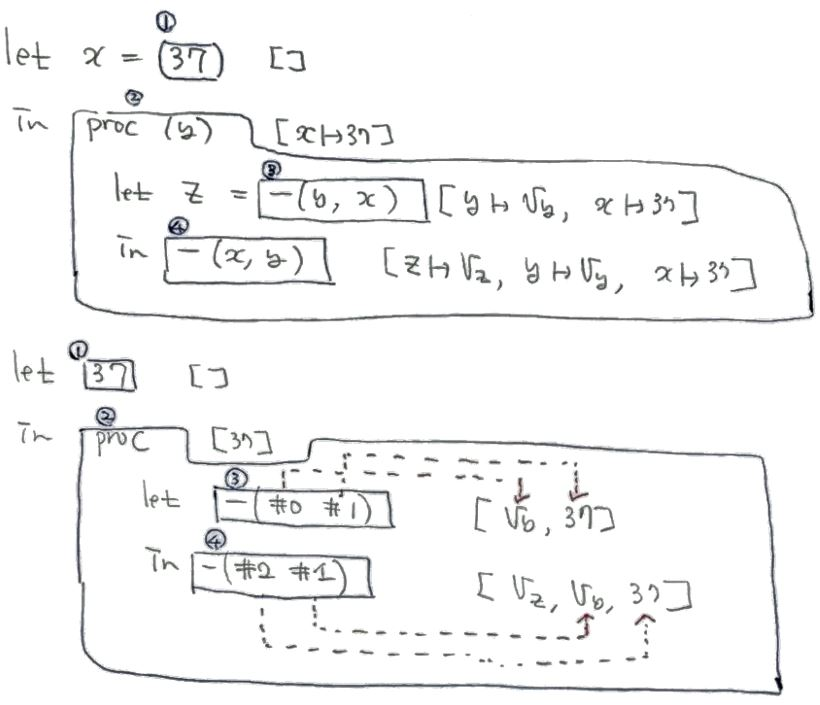
\includegraphics[width=0.75\linewidth]{fig_debruijn_indices}

%%%%%%%%%%%% Slide %%%%%%%%%%%%%%%%%%%%%%%%%%%%%%%%%%%%%%%%%%%%%%%%%%%
\heading{3.7 Implementing Lexical Addressing}

Implementation of the lexical address analysis: \al
let x = 37 \al
in proc (y) \al
\ \ \ let z = -(y,x) \ \ \ \ \ \ \ \ \ depth(y)=0, depth(x)=1 \al
\ \ \ in -(x,y) \ \ \ \ \ \ \ \ \ \ \ \ \ \ \ depth(x)=2, depth(y)=1 \al
\al
is translated into \al
\al
(a-program \al
\ \ \ (nameless-let-exp (const-exp 37) \al
\ \ \ (nameless-proc-exp \al
\ \ \ \ \ \ (nameless-let-exp \al
\ \ \ \ \ \ \ \ \ (diff-exp (nameless-var-exp 0) (nameless-var-exp 1)) \al
\ \ \ \ \ \ \ \ \ (diff-exp (nameless-var-exp 2) (nameless-var-exp 1)) \al

%%%%%%%%%%%% Slide %%%%%%%%%%%%%%%%%%%%%%%%%%%%%%%%%%%%%%%%%%%%%%%%%%%
\heading{3.7.1 The Translator}

A procedure translation-of-program that \al
- takes a program, \al
- removes all the variables from the declarations, and \al
- replaces every variable reference by its lexical depth.

cf. translation-of-program vs. value-of-program

Static environment: a list of variables, representing the scopes within
which the current expression lies. \al
- See Figure 3.15 \al
- cf. Senv vs. Env

Implementation: P.96 and Figure 3.16

%%%%%%%%%%%% Slide %%%%%%%%%%%%%%%%%%%%%%%%%%%%%%%%%%%%%%%%%%%%%%%%%%%
\heading{3.7.2 The Nameless Interpreter}

This interpreter takes advantage of the predictions of the lexical-address
analyzer to avoid explicitly searching for variables at runtime.

Nameless environment: a list of denoted values \al
- Figure 3.17 and the figure in P.98

Two modified procedures, value-of and value-of-program, 
with nameless environment \al
- Figure 3.18 and P.100

\end{huge}
\end{document}

%%%%%%%%%%%% Slide %%%%%%%%%%%%%%%%%%%%%%%%%%%%%%%%%%%%%%%%%%%%%%%%%%%
\heading{2.1 Specifying Data via Interfaces}
Every time we decide to represent a certain set of quantities in a particular way, we are defining a new data type  \al
- whose values are those representations and \al
- whose operations are the procedures manipulating those entities \al

Motivation\al
- The representation of these entities is often complex, so we do 
not want to be concerned with their details. \al 
- We may decide to change the representation of the data. \al
%- We may wish to develop a simple implementation first and then later change to make it efficient \al
- To change the representation of some data, we must be able to locate all parts of a program that are dependent on the representation.

%%%%%%%%%%%% Slide %%%%%%%%%%%%%%%%%%%%%%%%%%%%%%%%%%%%%%%%%%%%%%%%%%%
\heading{2.1 Specifying Data via Interfaces (cont.)}

Data abstraction:  \al
- a data type = an interface + an implementation \al
- {\it Abstract data type}

A client code is {\it representation-independent} if it only uses the interface.


%%%%%%%%%%%% Slide %%%%%%%%%%%%%%%%%%%%%%%%%%%%%%%%%%%%%%%%%%%%%%%%%%%
\heading{2.1 Specifying Data via Interfaces (cont.)}

Notation: the representation of data $v$, $\rep{v}$

A simple example: the (abstract) data type of natural numbers \al
- An interface
\begin{eqnarray*}
\mbox{(zero)} &=& \rep{0} 
\\
\mbox{(is-zero? $\rep{n}$)} & = &
	\left \{
	\begin{array}{l}
	\#t \ \ \ \ \ \ n = 0 \\
	\#f \ \ \ \ \ \ n \not=0
	\end{array}
	\right . 
\\
\mbox{(successor $\rep{n}$)} & = & 
\rep{n+1} \ \ \ \ \ \ (n\geq 0) 
\\
\mbox{(predecessor $\rep{n+1}$)} & = & 
\rep{n} \ \ \ \ \ \ (n\geq 0)  
\end{eqnarray*}

Many possible representations of the interface \al
- Unary representation \al
- Scheme number representation \al
- Bignum representation

%%%%%%%%%%%% Slide %%%%%%%%%%%%%%%%%%%%%%%%%%%%%%%%%%%%%%%%%%%%%%%%%%%
\heading{2.2 Representation Strategies for Data Types}

Some strategies for representing a data type of environments \al
- In a PL implementation, it associaes each variable with a value  \al
- In a compiler, it associates each variable with a type \al

Variables may be presented in any way so long as we can check two variables for equality. \al

From the next slides, \al
- The environment interface \al
- Data structure representation \al
- Procedural representation 

%%%%%%%%%%%% Slide %%%%%%%%%%%%%%%%%%%%%%%%%%%%%%%%%%%%%%%%%%%%%%%%%%%
\heading{The Environment Interface}

An environment is a function mapping a finite set of variables onto (Scheme) values \al
- $env = \{ (var_1,val1), \cdots, (var_n, valn) \}$. \al
- the value of the variable in {\it env} is called its {\it binding} in {\it env}.

The interface to a data type for environments \al
\begin{eqnarray*}
\mbox{(empty-env)} &=& \rep{\emptyset} 
\\
\mbox{(apply-env \ $\rep{f}$ \ {\it var})} &=& f(var)
\\
\mbox{(extend-env \ {\it var} \ {\it v} \ $\rep{f}$)} &=& \rep{g}
\\
& & \mbox{where} \ g(var_1) =
\left \{
\begin{array}{l}
v \ \ \ \ \ \ \mbox{if} \ var_1=var 
\\
f(var_1) \ \ \ \mbox{otherwise}
\end{array}
\right .
\end{eqnarray*}

%%%%%%%%%%%% Slide %%%%%%%%%%%%%%%%%%%%%%%%%%%%%%%%%%%%%%%%%%%%%%%%%%%
\heading{The Environment Interface (cont.)}

Using the interface, \al
- to build an environment: $env=\{(d,6), \ (x,7), \ (y,8) \}$ \al
\prompt (define env \al
\ \ \ \ \ 	(extend-env `d 6 \al
\ \ \ \ \ \ \ 		(extend-env `y 8 \al
\ \ \ \ \ \ \ \ \			(extend-env `x 7 \al
\ \ \ \ \ \ \ \ \ \ \ 				(extend-env `y 14 \al
\ \ \ \ \ \ \ \ \ \ \  \ \					(empty-env))))) \al \al
- to look up a binding for a variable: $env(d)$ \al
\prompt (apply-env env `d)

\ \\
Constructors and observers of the procedures of the interface \al

%%%%%%%%%%%% Slide %%%%%%%%%%%%%%%%%%%%%%%%%%%%%%%%%%%%%%%%%%%%%%%%%%%
\heading{Data Structure Representation}

Every environment can be built by starting with the empty environment 
and applying extend-env $n$ times.

So, every environment can be built by an expression in the following 
grammar:
%\mat{
\begin{eqnarray*}
Env\mm exp & ::= & (empty \mm env)\\
           & ::= & (extend \mm env \ Identifier \ Scheme \mm value \ Env \mm exp)
\end{eqnarray*}
%}
\al
- See an implementation in Figure 2.1

%%%%%%%%%%%% Slide %%%%%%%%%%%%%%%%%%%%%%%%%%%%%%%%%%%%%%%%%%%%%%%%%%%
\heading{Procedural Representation}

An alternative representation is to use procedures for environments. \al
- See an implementation in P.40

Every client-code using the environment interface will be 
represent-independent. \al
- One representation can be replaced with the other without affecting
the client code.

cf. {\it defunctionalization} \al
- A transformation of (higher-order) functions or a procedural representation
into data structures or data structure representation

%%%%%%%%%%%% Slide %%%%%%%%%%%%%%%%%%%%%%%%%%%%%%%%%%%%%%%%%%%%%%%%%%%
\heading{2.3 Interfaces for Recursive Data Types}

A recursive data type for lambda-calculus expressions:
%\mat{
\begin{eqnarray*}
Lc\mm exp 
 & ::= & Identifier \\
 & ::= & (lambda \ ( Identifier ) \ Lc\mm exp) \\
 & ::= & (Lc\mm exp \ Lc\mm exp)
\end{eqnarray*}
%}

What is an interface for the lambda-calculus expressions? 
In other words, what are constructors and observers for them? \al
- cf. Observers (predicates and extractors) \al

Using the interface, write a procedure as \al
- $occurs\mm free \ : \ Sym \ \times \ LcExp \ \rightarrow \ Bool$

%%%%%%%%%%%% Slide %%%%%%%%%%%%%%%%%%%%%%%%%%%%%%%%%%%%%%%%%%%%%%%%%%%
\heading{2.4 A Tool for Defining Recursive Data Types}

A tool for automatically constructing and implementing such interfaces
one discussed in Section 2.3 in Scheme: \al
(define-datatype lc-exp lc-exp? \al
\ \ \ (var-exp (var identifier?)) \al
\ \ \ (lambda-exp (bound-var identifier?)) \al
\ \ \ (app-exp (rator lc-exp?) (rand lc-exp?))) \al

Examples: \al
- $x$ : (var-exp `x) \al
- $\lambda x. x$ : (lambda-exp `x (var-exp `x)) \al
- $(lambda x. x) (lambda y.y)$ : \al
\ \ \ \ \ \ \ \ \ (app-exp \al
\ \ \ \ \ \ \ \ \ \ \ \ \ \ (lambda-exp `x (var-exp `x)) \al
\ \ \ \ \ \ \ \ \ \ \ \ \ \ (lambda-exp `y (var-exp `y)))

%%%%%%%%%%%% Slide %%%%%%%%%%%%%%%%%%%%%%%%%%%%%%%%%%%%%%%%%%%%%%%%%%%
\heading{2.4 A Tool for Defining Rec. Data Types(Cont.)}

A procedure occurs-free? using the interface generated by the tool. \al
- the form ``cases'' to determine the variant to which an object of a data type 
belongs and to extract its components. \al
(define occurs-free? \al
\ \ \ (lambda (search-var exp) \al
\ \ \ \ \ \ (cases lc-exp exp \al
\ \ \ \ \ \ \ \ \ (var-exp (var) (eqv? var search-var)) \al
\ \ \ \ \ \ \ \ \ (lambda-exp (bound-var body) \al
\ \ \ \ \ \ \ \ \ \ \ \ (and \al
\ \ \ \ \ \ \ \ \ \ \ \ \ \ \ (not (eqv? search-var bound-var)) \al
\ \ \ \ \ \ \ \ \ \ \ \ \ \ \ (occurs-free? search-var body))) \al
\ \ \ \ \ \ \ \ \ (app-exp (rator rand) \al
\ \ \ \ \ \ \ \ \ \ \ \ (or \al
\ \ \ \ \ \ \ \ \ \ \ \ \ \ \ (occurs-free? search-var rator) \al
\ \ \ \ \ \ \ \ \ \ \ \ \ \ \ (occurs-free? search-var rand))))))

%%%%%%%%%%%% Slide %%%%%%%%%%%%%%%%%%%%%%%%%%%%%%%%%%%%%%%%%%%%%%%%%%%
\heading{2.4 A Tool for Defining Rec. Data Types(Cont.)}

See the textbook (P.47 and P.49) for the general form define-datatype
declaration and the general syntax of cases. \al

The form ``define-datatype'' is an example of a {\it domain-specific 
language (DSL)}. \al
- A DSL is a small language for describing a single task among a small,
well-defined set of tasks.  \al
- Such a language may lie inside a general-purpose language, 
as define-datatype does, or 
it may be a standalone language with its own set of tools. 

%%%%%%%%%%%% Slide %%%%%%%%%%%%%%%%%%%%%%%%%%%%%%%%%%%%%%%%%%%%%%%%%%%
\heading{2.5 Abstract Syntax and Its Representation}

Concrete syntax (defined by a grammar) vs. 
Abstract syntax (by define-datatype) \al
- The concrete syntax is an external representation for humans \al
- The abstract syntax is an internal one for computers \al
- See Figure 2.2 for a comparison

Parsing is a task to derving the corresponding abstract syntax tree from
the concrete syntax which is a sequence of characters. \al
- Parser \al
- Parser generator \al
- $parse\mm expression : SchemeVal \rightarrow LcExp$

The reverse task of parsing is called unparsing or ``pretty-printing''. \al
- Unparser or pretty-printer \al
- $unparse\mm lc\mm exp : LcExp \rightarrow SchemeVal$



%%%%%%%%%%%% Slide %%%%%%%%%%%%%%%%%%%%%%%%%%%%%%%%%%%%%%%%%%%%%%%%%%%
\heading{Inductive Specification}

[Example] A top-down style inductive specification:\al\al
A natural number $n$ is in $S$ if and only if\al
\ \ \ 1. $n=0$ or\al
\ \ \ 2. $n-3 \in S$


%%%%%%%%%%%% Slide %%%%%%%%%%%%%%%%%%%%%%%%%%%%%%%%%%%%%%%%%%%%%%%%%%%
\heading{Inductive Specification (cont.)}

[Example] A bottom-up definition:\al\al
The set $S$ to be the smallest set contained in $N=\{0,1,2,\cdots\}$ and satisfying the following two properties:\al\al
\ \ \ 1. $0 \in S$, and \al
\ \ \ 2. if $n \in S$ then $n + 3 \in S$. 

[Example] Rules of inference:\al\al
The same set $S$ as above \al\al
%\mat{
\begin{tabular}{c}
\phantom{or }\\ \hline
$0 \in S$
\end{tabular}
 \ \ \ 
\begin{tabular}{c}
$n \in S$ \\ \hline
$(n+3) \in S$
\end{tabular}
%}

%%%%%%%%%%%% Slide %%%%%%%%%%%%%%%%%%%%%%%%%%%%%%%%%%%%%%%%%%%%%%%%%%%
\heading{Defining Sets Using Grammars}
Grammars\al
- Nonterminal symbols: the names of the sets being defined \al
- Terminal symbols: the characters in the external representation\al
- Production (rule)

Nonterminals = syntactic categories.

[Example]
%\mat{
\begin{eqnarray*}
List\mm of\mm int & ::= & ()\\
                & ::= & (Int \ . \ List\mm of\mm int)
\end{eqnarray*}
%}

cf. Variations of production rules

[Example] $S\mm list$, $S\mm exp$, $Bintree$, $LcExp$

%%%%%%%%%%%% Slide %%%%%%%%%%%%%%%%%%%%%%%%%%%%%%%%%%%%%%%%%%%%%%%%%%%
\heading{Defining Sets Using Grammars (cont.)}

The grammars are said to be {\it context-free} because a rule defining a given syntactic category may be applied in any context that makes reference to that syntactic category.

Sometimes we have to look at the context in which the production is applied. Such constraints are called {\it context-sensitive constraints} .\al
- E.g., in many languages every variable must be declared before it is used. 

In practice, the usual approach is first to specify a context-free grammar. Context-sensitive constraints are then added using other methods. 

%%%%%%%%%%%% Slide %%%%%%%%%%%%%%%%%%%%%%%%%%%%%%%%%%%%%%%%%%%%%%%%%%%
\heading{Induction}

We use the inductive definitions in two ways:\al
- to prove theorems about members of the set and\al
- to write programs that manipulate them.

%%%%%%%%%%%% Slide %%%%%%%%%%%%%%%%%%%%%%%%%%%%%%%%%%%%%%%%%%%%%%%%%%%
\heading{1.2 Deriving Recursive Programs}

We have seen that we can analyze an element of an inductively defined set to see how it is built from smaller elements of the set.

We use this idea to define/write a general procedure that compute on inductively defined sets.

When defining a procedure that operates on inductively defined data, the structure of the program should be patterned after the structure of the data.

%%%%%%%%%%%% Slide %%%%%%%%%%%%%%%%%%%%%%%%%%%%%%%%%%%%%%%%%%%%%%%%%%%
\heading{1.2 Deriving Recursive Programs (cont.)}

list-length determines the number of elements in a list: \al
\prompt (list-length `(a b c))\al
3\al
\prompt (list-length `((x) ())\al
2

nth-element picks the n-th element of a list:\al
\prompt (nth-element `(a b c d e) 3)\al
d

%%%%%%%%%%%% Slide %%%%%%%%%%%%%%%%%%%%%%%%%%%%%%%%%%%%%%%%%%%%%%%%%%%
\heading{1.2 Deriving Recursive Programs (cont.)}

remove-first:\al\al
\prompt (remove-first `a `(a b c))\al
(b c)\al
\prompt (remove-first `b `(e f g))\al
(e f g)\al
\prompt (remove-first `a4 `(c1 a4 c1 a4))\al
(c1 c1 a4)\al
\prompt (remove-first `x `())\al
()

%%%%%%%%%%%% Slide %%%%%%%%%%%%%%%%%%%%%%%%%%%%%%%%%%%%%%%%%%%%%%%%%%%
\heading{1.2 Deriving Recursive Programs (cont.)}

The procedure occurs-free? takes a variable {\it var}, and a lambda-calculus expression {\it exp}, and it determines whether or not {\it var} occurs free in {\it exp}. \al\al
\prompt (occurs-free? `x `x) \al
\#t \al
\prompt (occurs-free? `x `y) \al
\#f \al
\prompt (occurs-free? `x `(lambda (x) (x y))) \al
\#f \al
\prompt (occurs-free? `x `((lambda (x) x) (x y))) \al
\#t \al
\prompt (occurs-free? `x `(lambda (y) (lambda (z) (x (y z))))) \al
\#t

%%%%%%%%%%%% Slide %%%%%%%%%%%%%%%%%%%%%%%%%%%%%%%%%%%%%%%%%%%%%%%%%%%
\heading{1.2 Deriving Recursive Programs (cont.)}

The procedure {\it subst} takes three arguments: two symbols, {\it new} and {\it old}, and an s-list, {\it slist}. All elements of {\it slist} are examined, and a new list is returned that is similar to {\it slist} but with all occurrences of {\it old} replaced by instances of {\it new}.

\prompt (subst `a `b `((b c) (b () d))) \al
((a c) (a () d)


%%%%%%%%%%%% Slide %%%%%%%%%%%%%%%%%%%%%%%%%%%%%%%%%%%%%%%%%%%%%%%%%%%
\heading{1.3 Auxiliary Procedure and Context Arguments}

Auxiliary procedures\al
- number-elements-from\al
- number-elements\al
- list-sum\al
- partial-vector-sum\al
- vector-sum

\end{huge} 



